\documentclass{beamer}
\usetheme{focus}
\definecolor{main}{RGB}{92, 138, 168}
\definecolor{background}{RGB}{250, 250, 250}
\graphicspath{{graphics/}}

\title{Cache for HLS}
\subtitle{A multi-process architecture}
\author{Brignone Giovanni}
\titlegraphic{
\includegraphics[width=.4\textwidth]{polito_logo.png}}
\institute{Politecnico di Torino}
\date{June 7, 2021}

\begin{document}
\begin{frame}
	\maketitle
\end{frame}

\begin{frame}{Outline}
	\tableofcontents
\end{frame}

\section{Introduction}
\subsection{Motivation}
\begin{frame}{Motivation}
	\begin{itemize}
		\item \textbf{Problem}:\\
			big arrays are mapped to \underline{DRAM}, therefore they can be
			performance \underline{bottlenecks}
		\item \textbf{Proposed solution}:\\
			cache module storing data to fast \underline{BRAMs} to
			be integrated into any design with \underline{minimal effort}
	\end{itemize}
\end{frame}

\section{Architecture}
\subsection{Inlined architecture}
\begin{frame}{Inlined architecture (Ma Liang)}
	Accesses to cached array replaced with whole cache logic:
	\begin{itemize}
		\item straightforward implementation
		\item cache logic mixed with application logic
		\item single-port only
	\end{itemize}
\end{frame}
\subsection{Multi-process architecture}
\begin{frame}{Multi-process architecture}
	\begin{minipage}{.7\textwidth}
		Accesses to cached array replaced with request sending
		and response reception:
		\begin{itemize}
			\item decoupling between application and cache logic
				(communication through FIFOs only)
			\item may support multiple ports (work in progress)
		\end{itemize}
	\end{minipage}
	\begin{minipage}{.29\textwidth}
		\begin{center}
			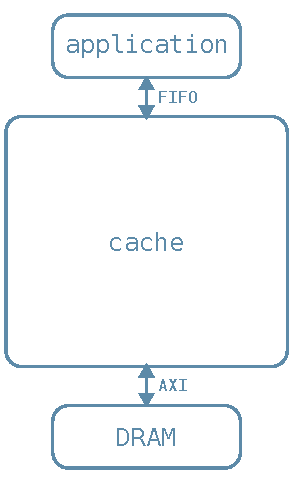
\includegraphics[width=.9\textwidth,height=.9\textheight,keepaspectratio]{complete_arch.pdf}
		\end{center}
	\end{minipage}
\end{frame}

\section{Implementation}
\subsection{Vitis HLS}
\begin{frame}{Vitis HLS (2020.2)}
	\begin{minipage}{.89\textwidth}
		\begin{itemize}
			\item \textbf{Relevant features}:
				\begin{itemize}
					\item multiple processes modeling:
						\begin{itemize}
							\item \underline{SW:} \texttt{std::thread}
							\item \underline{HW:} \texttt{DATAFLOW} with
								\textit{start propagation} disabled
						\end{itemize}
					\item \texttt{hls::stream} as FIFO implementation
					\item loop pipelining
					\item automatic port widening
				\end{itemize}
			\item \textbf{Limitations}:
				\begin{itemize}
					\item automatic \texttt{class} disaggregation
						prevents ``\texttt{[]}~operator''
						override for \texttt{set} operation\\
						(pointer to \texttt{class} is required)
				\end{itemize}
		\end{itemize}
	\end{minipage}
	\begin{minipage}{.1\textwidth}
		\begin{center}
			
\includegraphics[width=.9\textwidth]{vitislogo.png}
		\end{center}
	\end{minipage}
\end{frame}

\subsection{Internal architecture}
\begin{frame}{Internal architecture}
	\begin{minipage}{.7\textwidth}
	\begin{itemize}
		\item \textbf{Issue}: persuade HLS to schedule response writing
			to FIFO in case of HIT early in the pipeline
		\item \textbf{Solution}: split the cache into two processes:
			\begin{enumerate}
				\item \texttt{core}:
					\begin{itemize}
						\item manage requests from \texttt{application}
						\item keep cache data structures up-to-date
					\end{itemize}
				\item \texttt{mem\_if}:
					\begin{itemize}
						\item manage DRAM accesses
					\end{itemize}
			\end{enumerate}
			$\Rightarrow$ synthesizer job is simplified:\\
			if HIT, response is written in 1 cycle
	\end{itemize}
	\end{minipage}
	\begin{minipage}{.29\textwidth}
		\begin{center}
			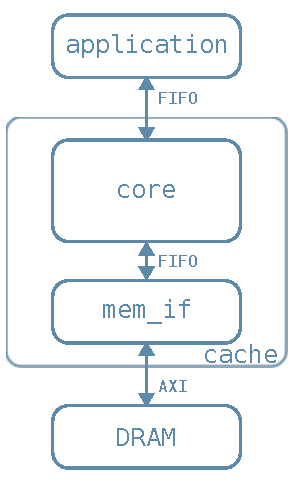
\includegraphics[width=.9\textwidth,height=.9\textheight,keepaspectratio]{internal_arch.pdf}
		\end{center}
	\end{minipage}
\end{frame}
\begin{frame}{\texttt{mem\_if} implementation}
	\begin{minipage}{.7\textwidth}
		Manage DRAM accesses:
		\begin{enumerate}
			\item read request from \texttt{core}
			\item access DRAM
			\item write response to \texttt{core}
				(if \texttt{read} request)
		\end{enumerate}
	\end{minipage}
	\begin{minipage}{.29\textwidth}
		\begin{center}
			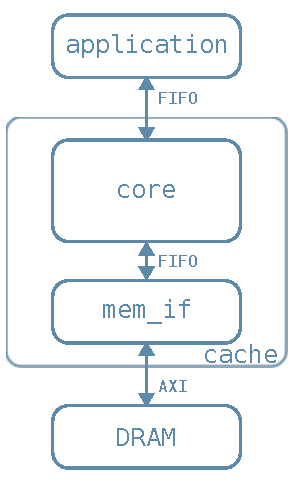
\includegraphics[width=.9\textwidth,height=.9\textheight,keepaspectratio]{internal_arch.pdf}
		\end{center}
	\end{minipage}
\end{frame}
\begin{frame}{\texttt{core} implementation}
	\begin{minipage}{.7\textwidth}
		Infinite pipelined loop performing following steps:
		\begin{enumerate}
			\item read request from \texttt{application}
			\item check if it is an HIT or a MISS
			\item if MISS: 
				\begin{itemize}
					\item if the cache line to be overwritten $\text{\texttt{line}}_{\text{old}}$
						has been modified, issue a \texttt{write}
						request of $\text{\texttt{line}}_{\text{old}}$ to \texttt{mem\_if}
					\item issue a \texttt{read} request of the
						requested line to \texttt{mem\_if}
					\item read \texttt{mem\_if} response and
						update BRAM

				\end{itemize}
			\item access BRAM
			\item write response to \texttt{application}
				(if \texttt{read} request)
		\end{enumerate}
	\end{minipage}
	\begin{minipage}{.29\textwidth}
		\begin{center}
			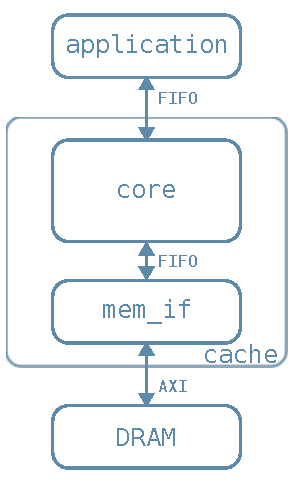
\includegraphics[width=.9\textwidth,height=.9\textheight,keepaspectratio]{internal_arch.pdf}
		\end{center}
	\end{minipage}
\end{frame}
\begin{frame}{\texttt{core} implementation}
	\begin{minipage}{.7\textwidth}
		\begin{itemize}
			\item \textbf{Problem}:
				reading BRAM immediately after it is written
				by the \texttt{fill} process causes an increase
				of II
			\item \textbf{Solution}:
				store the \texttt{mem\_if} response in a buffer
				which can be immediately accessed and update BRAM
				afterwards
		\end{itemize}
	\end{minipage}
	\begin{minipage}{.29\textwidth}
		\begin{center}
			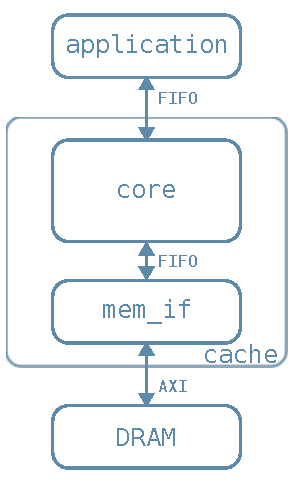
\includegraphics[width=.9\textwidth,height=.9\textheight,keepaspectratio]{internal_arch.pdf}
		\end{center}
	\end{minipage}
\end{frame}
\begin{frame}{\texttt{core} implementation}
	\begin{minipage}{.7\textwidth}
		\begin{itemize}
			\item \textbf{Problem}:
				reading BRAM immediately after it is written by
				a previous \texttt{write} request causes an
				increase of II
			\item \textbf{Solution}:
				insert a \texttt{raw\_cache} (single-line
				cache storing last written line): in case of a
				\texttt{read} request right after a \texttt{write}
				request to the same line, the access is performed
				to the \texttt{raw\_cache} instead of BRAM
		\end{itemize}
	\end{minipage}
	\begin{minipage}{.29\textwidth}
		\begin{center}
			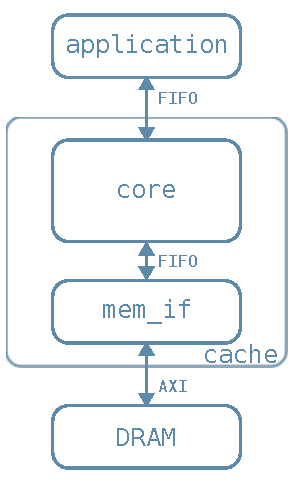
\includegraphics[width=.9\textwidth,height=.9\textheight,keepaspectratio]{internal_arch.pdf}
		\end{center}
	\end{minipage}
\end{frame}
\begin{frame}{Request optimization}
	\begin{minipage}{.7\textwidth}
		\begin{itemize}
			\item \textbf{Scenario}:
				\begin{itemize}
					\item each FIFO access costs 1 cycle
					\item accesses to arrays are often sequential
				\end{itemize}
			\item \textbf{Proposed solution}:\\
				insert a \texttt{l1\_cache} in the interface,
				on \texttt{application} side: a \texttt{read} request
				gets the whole cache line, stores it and returns the
				required element; if subsequent requests read the same
				line, the interface can immediately return data, avoiding
				sending any request and waiting for response
		\end{itemize}
	\end{minipage}
	\begin{minipage}{.29\textwidth}
		\begin{center}
			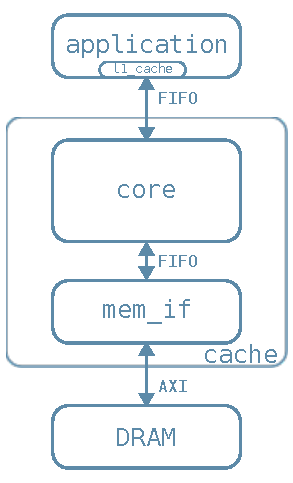
\includegraphics[width=.9\textwidth,height=.9\textheight,keepaspectratio]{l1_arch.pdf}
		\end{center}
	\end{minipage}
\end{frame}

\section{Future work}
% multi-ports (possibly in RTL)

\end{document}

